\documentclass{standalone}
\usepackage{pgfplots}
\usepackage{fontspec}
\usepackage{graphicx}
\usepackage{amsmath, soul,multirow}
\usepackage{mathtools}
\usepackage{booktabs}
\usepackage{enumitem}
\usepackage{marvosym}
\usepackage{rotating}
\usepackage{amsmath,blkarray}
\pagestyle{empty}
\usepackage[normalem]{ulem}
%\usepackage{tikz}
\usetikzlibrary{arrows, backgrounds, fit, shapes.misc}
\setmainfont{Humor Sans}

\newcommand{\horizontal}[1]{\textrm{\begin{turn}{-90} #1 \end{turn}}}

\newcommand\irregularcircle[2]{% radius, irregularity
  \pgfextra {\pgfmathsetmacro\len{(#1)+rand*(#2)}}
  +(0:\len pt)
  \foreach \a in {10,20,...,350}{
    \pgfextra {\pgfmathsetmacro\len{(#1)+rand*(#2)}}
    -- +(\a:\len pt)
  } -- cycle
}

\begin{document}

\tikzstyle{block} = [draw=none,inner sep=0pt]
\tikzstyle{line} = [draw, thick,-latex']
\begin{tikzpicture}[node distance = 4cm,auto]

	\node[block] (raw-data) 
	{
		\begin{minipage}{0.5\textwidth}
			{\small
			\begin{enumerate}
				\item[] \uline{Scientific text}
				\item[] {\color{blue} Scientific Discovery}
				\item[] Contradictory discovery
				\item[] {\color{red} Different discovery}
			\end{enumerate}
		}
		\end{minipage}
	}; 

	\node[block,right of=raw-data, right=0cm] (processed-data)
	{	

	\begin{minipage}{0.4\textwidth}
		\[
		\begin{array}{ccccc}
			& \multicolumn{4}{c}{\textrm{\uline{word count} }\rightarrow} \\
			 & \horizontal{Science} & \horizontal{Discover} & \vdots & \horizontal{Tenure} \\
\multirow{5}{*}{\begin{turn}{-90} \textrm{\uline{articles}} $\rightarrow$ \end{turn}}
		& \textrm{\color{red}20} & \textrm{\color{red}5} & \textrm{\color{red} 90} & \textrm{\color{red}4} \\
		& \textrm{\color{gray}30} & \textrm{\color{gray}70} & \textrm{\color{gray}6} & \textrm{\color{gray}12} \\
		&  & \vdots & \vdots &  \\
		& \textrm{\color{blue}50} & \textrm{\color{blue}10} & \textrm{\color{blue}3} & \textrm{\color{blue}20} \\
		& \textrm{5} & \textrm{100} & \textrm{30} & \textrm{2} \\
		\end{array}
	\]
	\end{minipage}
	};

	\node[block,below of=processed-data, below=0em] (non-orthogonal) 
	{
		\begin{minipage}{0.4\textwidth}
			\begin{tikzpicture}[dot/.style={circle,inner sep=2pt,fill,color=#1}]

				\node[dot=blue] at (0.5,0.5) {};
				\node[dot=red] at (0.9,1.1) {};
				\node[dot=black] at (0.6,0.6) {};
				\node[text width=7em] at (3,1.5) {\small No distance metric from LDA; topics \uline{not} orthogonal \\ };
				\draw[thick,->] (0,0) --node[below, below=0.5em] {\begin{turn}{10}Topic 1\end{turn}} (1.5,.35);
				\draw[thick,->] (0,0) --node[left, left=0.5em] {\begin{turn}{80} Topic 2\end{turn}} (.15,1.5);
			\end{tikzpicture}		
		\end{minipage}
	};

   \node[below of=raw-data] (orthogonal)
	{
		\begin{minipage}{0.3\textwidth}
			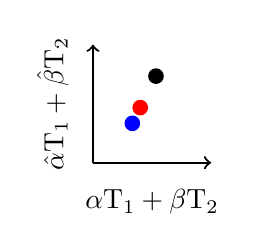
\begin{tikzpicture}[dot/.style={circle,inner sep=2pt,fill,color=#1}]

				\node[dot=blue] at (0.5,0.5) {};
				\node[dot=red] at (0.6,.7) {};
				\node[dot=black] at (0.8,1.1) {};
				\draw[thick,->] (0,0) --node[below right, below=0.6em] {$\alpha \textrm{T}_1+\beta\textrm{T}_2$} (1.5,0);
				\draw[thick,->] (0,0) --node[left, left=0.5em] {\begin{turn}{90} $\hat{\alpha} \textrm{T}_1+\hat{\beta}\textrm{T}_2$\end{turn}} (0,1.5);
			\end{tikzpicture}		
		\end{minipage}
	};

 	\draw[line] (raw-data) --node[above]{NLP} (processed-data);
	\draw[line] (processed-data) --node[right]{LDA} (non-orthogonal);
	\draw[line] (non-orthogonal) --node[above]{PCA} (orthogonal);
\end{tikzpicture}
\end{document}